\documentclass[conference]{IEEEtran} 
\IEEEoverridecommandlockouts
\usepackage{epsfig,graphicx,subcaption}
% \usepackage[hyphens]{url}
\usepackage{hyperref}


%\documentclass[a4paper,10pt]{article}
\usepackage[utf8]{inputenc}
\usepackage{times}

%opening
\title{VITAL: Vulnerability Injection via Taint AnaLysis
  \thanks{This work is sponsored by the Assistant Secretary of Defense
    for Research \& Engineering under Air Force Contract
    \#FA8721-05-C-0002.  Opinions, interpretations, conclusions and
    recommendations are those of the author and are not necessarily
    endorsed by the United States Government.} }

\author{
\IEEEauthorblockN{Brendan Dolan-Gavitt\IEEEauthorrefmark{1}, Patrick Hulin\IEEEauthorrefmark{2}, Tim Leek\IEEEauthorrefmark{2}, Ryan Whelan\IEEEauthorrefmark{2}}
\\
\small (Authors listed alphabetically) \\
\\
\IEEEauthorblockA{\IEEEauthorrefmark{1}NYU\\brendandg@nyu.edu}
\IEEEauthorblockA{\IEEEauthorrefmark{2}MIT Lincoln Laboratory\\
\{patrick.hulin,tleek,rwhelan\}@ll.mit.edu}
}

\begin{document}

\maketitle

\begin{abstract}

Work on automating vulnerability discovery has long been hampered by a shortage of ground-truth corpora with which to evaluate tools and techniques.
To begin to address this, we present VITAL, a system for automatically and quickly injecting large numbers of realistic bugs into program source code.  
VITAL employs a pair of taint-based measures to identify program quantities that both depend upon specific input bytes in a simple way yet do not overly influence control flow.
These DUAs (dead-uncomplicated and available data) are employed, via source-to-source transformation, to perturb program quantities at later program points that are likely to cause vulnerabilities.
Every VITAL vulnerability is accompanied by a fuzzed input that triggers it, whereas normal inputs are extremely unlikely to do so.
Further, every VITAL bug is validated, and thus every working bug comes with both a proof-of-concept input and a known manifestation point.  
These vulnerabilities are synthetic but, we argue, still realistic, in the sense that they are embedded deep with programs and are triggered by inputs.
In order for an automated tool to discover them, it would have to be able to reason correctly and precisely about all the code executed up to the DUA.
Using VITAL, we have injected tens of thousands of bugs into popular programs such as file, strings, readelf, tshark, and eog.
We believe VITAL can form the basis of an approach for generating extremely high quality ground truth vulnerability corpora, on demand.



\end{abstract}

\section{Motivation}
\label{sec:motivation}
\label{sec:motivation}

Bug-finding tools have been an active area of research for almost as long as computer programs have existed. 
Techniques such as abstract interpretation, fuzzing, and symbolic execution with constraint solving have been proposed, developed, and applied.
But evaluation has been a problem, as  ground truth is in extremely short supply.
Vulnerability corpora exist~\cite{Kass:2005} but they are of limited utility and quantity.
These corpora fall into two categories: historic and synthetic.
Corpora built from historic vulnerabilities contain too few examples to be of much use~\cite{Zitser:2004}.
However, these are closest to what we want to have since the bugs are embedded in real code, use real inputs, and are often well annotated with precise information about where the bug manifests itself.
The author's own experience creating such a corpus was that it is a difficult and lengthy process; a corpus of only fourteen very well annotated historic bugs with triggering inputs took about six months to construct. 
In addition, public corpora have the disadvantage of already being released, and thus rapidly become stale.
We can expect tools to have been trained to detect bugs that have been released.
Given the commercial price tag of new exploitable bugs, which is widely understood to begin in the mid five figures~\cite{Tsyrklevich:2015}, it is hard to find real bugs for our corpus that have not already been used to train tools.
And, while synthetic code stocked with bugs, auto-generated by scripts, can provide large numbers of diagnostic examples, each is only a tiny program and the constructions are often considered unrepresentative of real code~\cite{Kratkiewicz:2005,Juliet:2012}.

In practice, a vulnerability discovery tool is typically evaluated by running it and seeing what it finds. 
Thus, one technique is judged superior if it finds more bugs than another.
While this state of affairs is perfectly understandable, given the scarcity of ground truth, it is an obstacle to science and progress in vulnerability discovery.
There is currently no way to measure fundamental figures of merit such as miss and false alarm rate for a bug finding tool.

We propose the following requirements for bugs in a vulnerability corpus, if it is to be useful for research, development, and evaluation.
Bugs must

\begin{enumerate}
\item Be cheap and plentiful
\item Span the execution lifetime of a program
\item Be embedded in representative control and data flow
\item Come with an input that serves as an existence proof 
\item Manifest for a very small fraction of possible inputs
\end {enumerate}

\noindent
The first requirement, if we can meet it, is highly desirable since it enables frequent evaluation and hill climbing. 
Corpora are more valuable if they are essentially disposable. 
The second and third of these requirements stipulate that bugs must be realistic.
The fourth means the bug is demonstrable and serious, and is a precondition for determining exploitability. 
The fifth requirement is crucial.
Consider the converse: if a bug manifests for all or a large fraction of inputs it is trivially discoverable by simply running the program.

The approach we propose is to create a synthetic vulnerability via a few judicious and automated edits to the source code of a real program.
We will detail and give results for an implementation of this approach that satisfies all of the above requirements.
We call this implementation LAVA for Large-scale Automated Vulnerability Addition.    
A serious bug such as a buffer overflow can be injected by LAVA into a program like \verb+file+, which is 13K LOC, in about a 15 seconds.
LAVA bugs manifest all along the execution trace, in all parts of the program, shallow and deep, and make use of mostly completely normal data flow.
By construction, a LAVA bug comes with an input that triggers it, and no other input can have this effect upon the program.


\section{Scope}
\label{sec:scope}

We restrict our attention, with LAVA, to the injection of bugs into source code.
This makes sense given our interest in using it to assemble large corpora for the purpose of evaluating and developing vulnerability discovery techniques and systems.
Automated bug discovery systems can work on source
code~\cite{Cadar:2008, Ganesh:2009, Haller:2013, Yamaguchi:2014} or on
binaries~\cite{Cha:2012, Wang:2010};
we can easily test binary analysis tools by simply compiling the modified source.
Injecting bugs into binaries or byte code directly may also be possible using an approach similar to ours, but we do not consider that problem here.
We further narrow our focus to Linux open-source software written in C, due to the availability of source code and source rewriting tools.
As we detail later, a similar approach will work for other languages.

We want the injected bugs to be serious ones, i.e., potentially exploitable.
As a convenient proxy, our current focus is on injecting code that can result in out-of-bounds reads and writes that can be triggered by an attacker-controlled input; in Section~\ref{sec:future} we consider extensions to LAVA to support other bug classes.
We produce a proof-of-concept input to trigger any bug we successfully inject, although we do not attempt to produce an actual exploit.


\section{VITAL Overview}
\label{sec:overview}

At a high level, LAVA adds bugs to programs in the following manner.

\begin {enumerate}
\item Identify source code locations where input bytes that do not determine control flow and are still close to their original form are available. 
We call these quantities DUAs, for dead, uncomplicated and available. 
\item Find potential attack points that are temporally after a DUA in the program trace.
Attack points are source code locations where a DUA might be used, if only it were available there as well, to make a program vulnerable. 
\item Add code to the program to make the DUA value available at the attack point and use it to create the vulnerability. 
\end{enumerate}

These three steps are depicted in Figure~\ref{lava-picture} and will be discussed in the following three sections,
which refer to the worked example in Figure~\ref{worked-example}.


\begin{figure} 
\begin{tabular}{ll}
1 & \verb+ void foo(int a, int b, int c) {+ \\
2 & \verb-   int d=a+b+c;- \\
3 & \verb+   if (a == 0xdeadbeef) return;+ \\ 
4 & \verb+   memcpy(d,s,n);+ \\
5 & \verb_   // BUG_ \\
6 & \verb_   // memcpy(d+(b==0x666666)*b,s,n);_ \\
7 & \verb+ }+ \\
\end{tabular}
\caption{
LAVA worked example.  
a, b, and c are direct copies of input bytes at the start of function foo.
a is bytes 0..3, b is 4..7, and c is 8..11.
The value in b at the call to memcpy has tcn=0 and liveness=0,
so it can be used to trigger and control a vulnerability there.
}
\label{worked-example}
\end{figure}



\subsection {The DUA}

In a little more detail, the first step, in which DUAs are identified, is accomplished as follows.  

The program is executed under a dynamic taint analysis for a specific input.
That taint analysis has a few important features.
\begin{itemize}
\item Each individual byte in the input is given its own label.
Thus, if an internal program quantity is tainted and a direct copy of input bytes, then we can map that quantity back to a specific part of the input.  
\item The taint analysis operates, effectively, upon an LLVM version of the machine code for a program, including its libraries.
This means taint is propagated accurately and completely, even through esoteric x86 machine instructions like MMX and XMM.
\item The taint analysis keeps track of a \emph{set} of labels per input byte, meaning that it can represent computation that mixes input bytes.
\end{itemize}
We use the PANDA system to perform this taint analysis, with two crucial conceptual extensions in the form of taint-based measures.

The \emph{taint compute number} is a measure of how complicated a function of input bytes a tainted internal program quantity is.
TCN is illustrated in Figure~\ref{figure:taint-compute-number}; it simply tracks the depth of the tree of computation required to obtain 
a quantity from input bytes.
The smaller TCN is for a program quantity, the closer it is, computationally, to the input.
If TCN is 0, the quantity is a direct copy of input bytes.
The intuition behind this measure is that we need DUAs that are computationally close to the input in order to be able to use them with predictable results.
Note that TCN is not an ideal measure.
There are obviously situations in which the tree of computation is deep but the resulting DUA value is both completely predictable and has as much entropy as the original value.
However, TCN has the advantage that it is easy to compute.
Whenever the taint system needs to union label sets to represent computation, the TCN associated with the resulting set is one more than the max of those of the 
input sets.
TCN is an integer attached to the taint label set associated with each byte in a program.

The other taint-based measure LAVA introduces is \emph{liveness}, which is associated with taint labels, i.e. the input bytes themselves.
This is a straightforward accounting of how many branches a byte in the input has been used to decide.
Thus, if a particular input byte label was never found in a taint label set associated with any byte used in a branch, it will have liveness of 0.
A DUA entirely consisting of bytes with 0 or very low liveness can be considered \emph{dead} in the sense that it has very little influence upon control flow for this program trace.
If one were to fuzz dead bytes, the program should be indifferent and execute the same trace.  

The combination of uncomplicated (low TCN) and dead (low liveness) is a powerful one for vulnerability injection.
The DUAs it identifies are internal program quantities that are often a direct copy of input bytes, and which can be set to any chosen value without sending the program along a different path.  
These make very good triggers for vulnerabilities.

In the worked example, consider the variables \verb+x+ and \verb+y+ in lines 3 and 4, respectively.
These have TCNs of 0 and 1, respectively, and liveness 0. 
These are tainted values that will make idea DUAs.

\subsection {The attack point}

Attack point identification is a function of the type of vulnerability to be injected.
If the goal is to inject a memory read overflow, then reads via pointer dereference, array index, and bulk memory copy, e.g., are reasonable attack points.  
If the goal is to inject divide-by-zero, then arithmetic operations involving division will be attacked. 
Alternately, the goal might be to control one or more arguments to a library function.
The only requirement is that the attack point be parameterized in order that it be attackable when the DUA is made available there. 

For instance, in Figure~\ref{worked-example}, on line 12, the call to \verb+memcpy+ can be attacked by introducing a data-flow relation between either \verb+x+ or \verb+y+ 
and any of the arguments to \verb+memcpy+.

\subsection {Data-flow bug injection}

The third and final step to LAVA bug injection is introducing a dataflow relationship between DUA and attack point.  
If the DUA is in scope at the attack point then it can simply be used at the attack point to introduce the vulnerability.
If it is not in scope, new code is added to copy the DUA off into a safe place (perhaps in a data structure or a global), and also retrieve it and  make use of it value at the attack point. 
However, in order to ensure that the bug only manifest itself very occasionally, we must introduce a guard requiring that the DUA match a specific value if it is to be used to manifest the vulnerability.

In the worked example in Figure~\ref{worked-example}, the DUA \verb+x+ is still in scope at the \verb+memcpy+ attack point and
 the only source code modification necessary is to make use of it to introduce the vulnerability if it matches a particular value.  











\section{Implementation}
\label{sec:implementation}

\begin{figure}
\centering
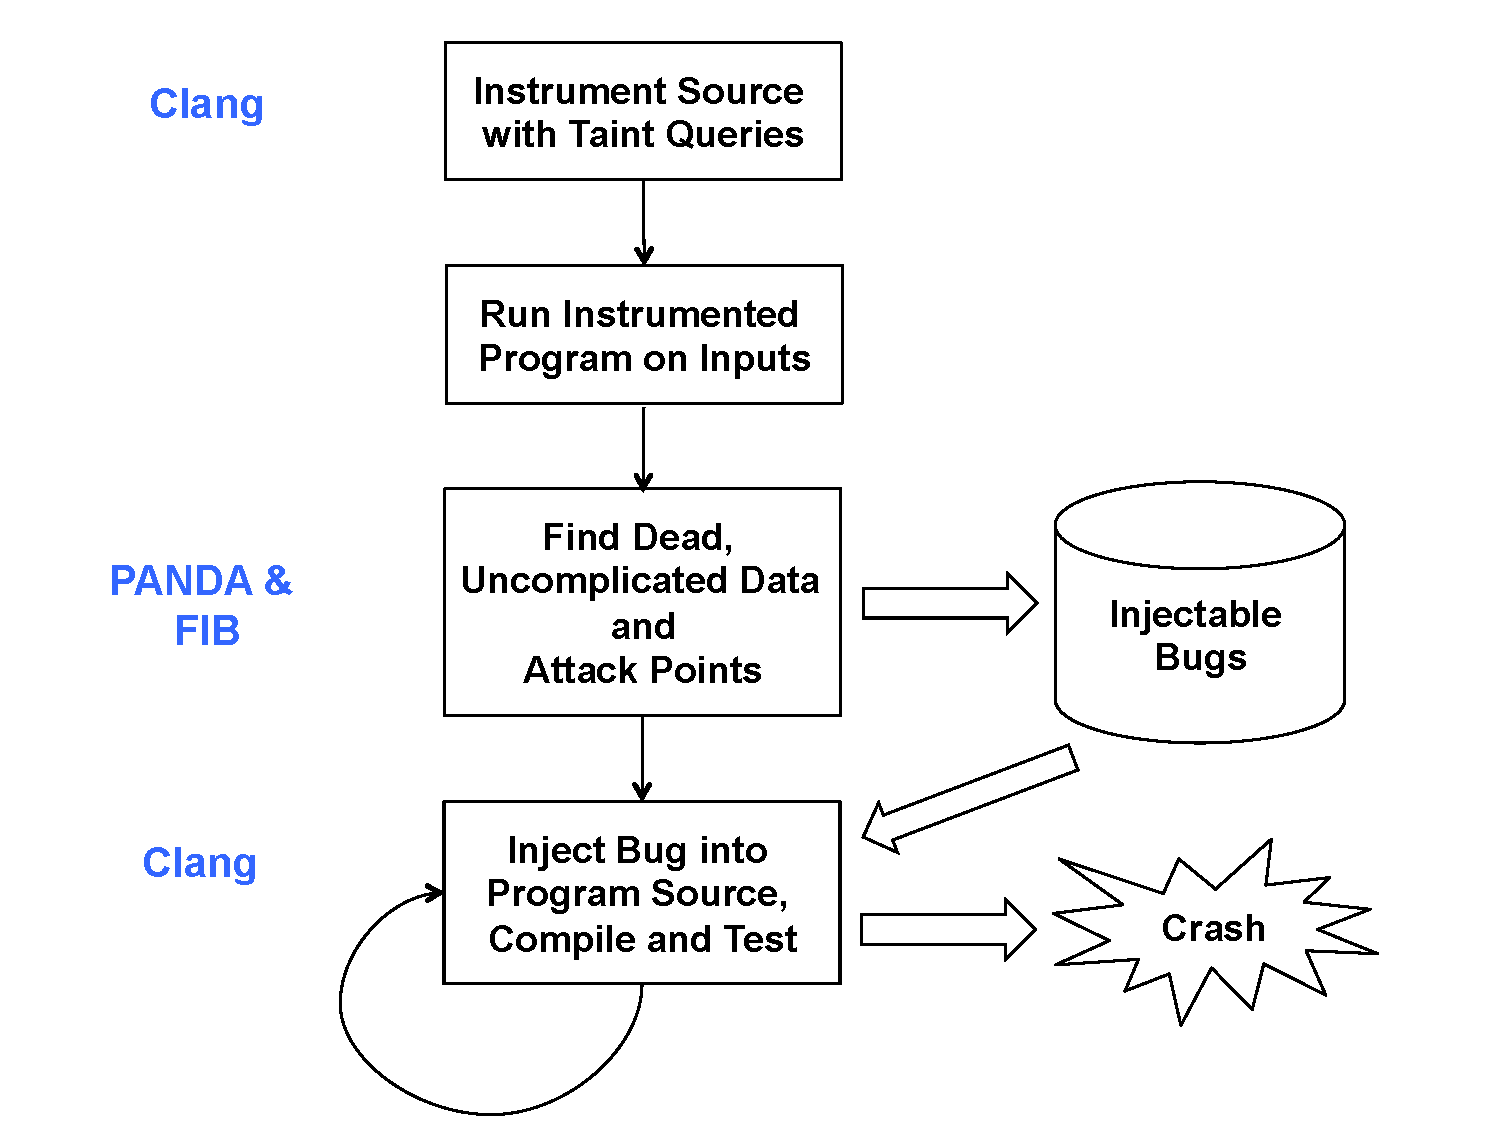
\includegraphics[width=3in]{lava-arch.pdf}
\caption{LAVA Implementation Architecture.  PANDA and Clang  are used to perform a dynamic taint analysis which identifies potential bug injections as DUA attack point pairs.
Each of these is validated with a corresponding source code change performed by Clang  as well.
Finally, every potentially buggy binary is tested against a targeted input change to determine if a buffer overflow actually results.}
\label{fig:lava-impl}
\end{figure}


The LAVA implementation operates in four stages to inject and validate buffer overflow vulnerabilities in Linux C source code. 

\begin{enumerate}
\item Compile a version of the target program which has been instrumented with taint queries.
\item Run the instrumented version against various inputs, tracking taint, and collecting taint query results and attack point information.
\item Mine the taint results for DUAs and attack points, and collect a list of potential injectable bugs.
\item Recompile the target with the relevant source code modifications for a bug, and test to see if it was successfully injected.
\end{enumerate}

These stages are also depicted in Figure~\ref{fig:lava-impl}

\subsection{Taint queries}
LAVA's taint queries rely on the PANDA dynamic analysis platform~\cite{PANDA}, which is based on the QEMU whole-system emulator.
PANDA augments Qemu in three important ways.
First, it introduces deterministic record and replay, which can be used for iterated and expensive analyses that cannot be performed online.
Second, it has a simple but powerful plugin architecture that allows for powerful analyses to be built and even built upon one another.
Third, it integrates, from S2E~\cite{S2E}, the ability to lift QEMU's intermediate language to LLVM for analysis.
The main feature of PANDA used by LAVA is a fast and robust dynamic taint analysis plugin that works upon the LLVM version of each 
basic block of emulated code.
This LLVM version includes emulated versions of every x86 instruction that QEMU supports.
QEMU often implements tricky processor instructions (e.g. MMX and XMM on x86) in C code.
These are compiled to LLVM bitcode using Clang, and, thereby made available for taint analysis by PANDA.
LAVA employes a simple PANDA plugin \verb+file_taint+ that is able to apply taint labels to bytes read from files in Linux.
This plugin, in turn, leverages operating system introspection and system call plugins in PANDA to determine the start file offset of the read as well as the number of bytes actually read.
This is how LAVA can make use of taint information that maps internal program quantities back to file offsets.  
% PANDA tracks taint between processes and the kernel.
Before running a target program under PANDA, LAVA first invokes a Clang plugin to insert taint queries into the source before and after function calls.
Each function argument is deconstructed into constituent lvals, and, for each, Clang adds a taint query as a \emph{hypervisor call} which notifies PANDA to query the taint system about a specific source-level variable.
The function return value also gets a taint query hypercall.
LAVA also uses Clang to insert source hypervisor calls at potential attack points.

\subsection{Running the program}
Once the target has been instrumented with taint queries, we run it against a variety of inputs.
Since our approach to gathering data about the program is fundamentally dynamic, we must take care to choose inputs to maximize code coverage.
To run the program, we load it as a virtual CD into a PANDA virtual machine and send commands to QEMU over a virtual serial port to execute the program against the input.
As the hypervisor calls in the program execute, PANDA logs results from taint queries and attack point encounters to a binary log file, the \emph{pandalog}.
Note that, because the pandalog is generated by hypercalls inserted into program source code, it can connect source-level information like variable names and source file locations to the taint queries and attack points.
This allows bug injection, later, to make use of source-level information. 


\begin{figure}
\lstinputlisting[language=Python,
        numbers=left, numberstyle=\tiny, stepnumber=2, numbersep=5pt,
        basicstyle=\ttfamily\footnotesize]{fib.py}
\caption{Python-style pseudocode for FIB. 
Panda log is processed in temporal order and the results of taint queries on values and branches are 
used to update the current set of DUAs and input byte liveness.
When an attack point is encountered, all currently viable DUAs are considered as potential data sources to inject a bug.}
\label{alg:fib}
\end{figure}

\subsection{Mining the Pandalog}
\label{sec:mining}
We then analyze the pandalog in temporal order, matching up DUAs with attack points to find potentially injectable bugs.
The program that does this is called \verb+FIB+ for ``find injectable bugs'', and is detailed in Figure~\ref{alg:fib}.
\verb+FIB+ considers the pandalog entries in temporal order.
Taint query entries are handled by the function \verb+collect_duas+ which maintains a set of currently viable DUAs.
Viable DUAs must have enough tainted bytes, and those bytes must be below some threshold for taint set cardinality and TCN.
Additionally, the liveness associated with all the input bytes which taint the DUA must be below a threshold.
Note that a DUA is associated with a specific program point and variable name, and only the last encountered DUA is retained in the viable set. 
This means that, if a DUA is a variable in a loop or in a function that is called many times, the set will only have one entry (the last) for that variable and source location, thus ensuring that value is up to date and potentially usable at an attack point.  
Tainted branch information in the pandalog updates liveness for all input bytes involved, in the function \verb+update_liveness+.
When \verb+FIB+ encounters an attack point in the pandalog, the function \verb+collect_bugs+ considers each DUA in the set,
and, those that are still viable with respect to liveness, are paired with the attack point as a potentially injectable bugs.
In the current implementation of LAVA, an attack point is an argument to a function call that can be \emph{made vulnerable by adding a DUA to it}.
This means the argument can be a pointer or some kind of integer type. 
The hope is that changing this value by a large amount may trigger a buffer overflow. 

\begin{figure}
\lstinputlisting[language=C,numbers=left, numberstyle=\tiny, stepnumber=2, numbersep=5pt,
        basicstyle=\ttfamily\footnotesize]{inj-example-dua-siphon.c}
\caption{PANDA taint analysis and the \texttt{FIB} algorithm determines that the first four bytes of \texttt{buf} are suitable for use in creating a bug.
This is the code injected by Clang into file's \texttt{src/encodings.c} to copy DUA value off for later use.}
\label{src:dua-siphon}
\end{figure}

\begin{figure}
\lstinputlisting[language=C,numbers=left, numberstyle=\tiny, stepnumber=2, numbersep=5pt,
        basicstyle=\ttfamily\footnotesize]{inj-example-attack.c}
\caption{Code injected into file's \texttt{src/readcdf.c} to use DUA value to create a vulnerability}
\label{src:dua-use}
\end{figure}

\subsection{Inject and Test Bugs}
For each DUA/attack point pair, we generate the C code which uses the DUA to trigger the bug using another Clang plugin.
At the source line and for the variable in the DUA, we inject code to copy its value into a static variable held by a helper function.
At the attack point, an argument to a function call, we insert code that retrieves the DUA value, determines if it matches a magic value, and if so adds it to one of the argument.
The final step in LAVA is simply compiling and testing the modified program on a proof-of-concept input file, in which the input file bytes indicated as tainting the DUA have been set to the correct value.
An example of the pair of source code insertions plus the file modifiction in order to inject a bug into the program \verb+file+ can be seen in Figures~\ref{src:dua-siphon}, and~\ref{src:dua-use}.
The original input to \verb+file+ was the binary \verb+/bin/ls+, and the required modification to that file is to simply set its first four bytes to the string 'lava' to trigger the bug. 
Note that the taint analysis and FIB identifies a DUA in one compilation unit and an attack point in another compilation unit.  


\section{Results}
\label{sec:results}
\label{section:results}

\begin{table*}[t]
\caption{LAVA Injection results for open source programs of various sizes}
\centering\footnotesize
\begin{tabular}{c|c|c|c|c|c|c|c|c|c}
        &         & Num       & Lines     &        &        & Potential & Validated  &         & Inj Time \\
Name    & Version & Src Files & C code    & N(DUA) & N(ATP) & Bugs      & Bugs       & Yield   & (sec)  \\\hline
file    & 5.22    & 19        & 10809     & 631    & 114    & 17518     & 774        & 38.7\%  & 16         \\  %    files verified.  sloc recomputed
%eog    & 3.4.2   &           & 22997     &        &        &           &            &         &         \\ 
readelf & 2.25    & 12        & 21052     & 3849   & 266    & 276367    & 1064       & 53.2 \% & 354     \\  % time verified.  files verified. sloc recomputed
bash    & 4.3     & 143       & 98871     & 3832   & 604    & 447645    & 192        & 9.6\%   & 153     \\  % time verified.  
tshark  & 1.8.2   & 1272      & 2186252   & 9853   & 1037   & 1240777   & 354        & 17.7\%  & 542     \\
\end{tabular} 
%For each, a single input file was used to perform a taint analysis with PANDA.
%Various program and dynamic trace statistics are reported as well as DUA, attack point (ATP), and yield (fraction of injected bugs that result in a segmentation violation).}
\label{table:insertion-results}
\end{table*}

We evaluated LAVA in three ways.
First, we injected large numbers of bugs into four open source programs: file, readelf (from binutils), bash, and tshark (the command-line version of the packet capture and analysis tool Wireshark).
For each of these, we report various statistics with respect to both the target program and also LAVA's success at injecting bugs.
Second, we evaluated the distribution and realism of LAVA's bugs by proposing and computing various measures.
Finally, we performed a preliminary investigation to see how effective existing bug-finding tools are at finding LAVA's bugs, by measuring the detection rates of an open-source fuzzer and a symbolic execution-based bug finder.

\subsection*{Counting Bugs}

Before we delve into the results, we must specify what it is we mean by an injected bug, and what makes two injected bugs distinct. Although there are many possible ways to define a bug, we choose a definition that best fits our target use case: two bugs should be considered different if an automated tool would have to reason about them differently. For our purposes, we define a bug as a unique pair $(DUA, attack point)$. Expanding this out, that means that the source file, line number, and variable name of the DUA, and the source file and line number of the attack point must be unique.

Some might object that this artificially inflates the count of bugs injected into the program, for example because it would consider two bugs distinct if they differ in where the file input becomes available to the program, even though the same file input bytes are used in both cases. 
But in fact these should be counted as different bugs: the data and control flow leading up to the point where the DUA occurs will be very different, and vulnerability discovery tools will have to reason differently about the two cases.

\subsection{Injection Experiments}
\label{sec:results:subsec:injection}

The results of injecting bugs into open source programs are summarized in Table~\ref{table:insertion-results}.
In this table, programs are ordered by size, in lines of C code, as measured by David Wheeler's \verb+sloccount+.
A single input was used with each program to measure taint and find injectable bugs.
The input to \verb+file+ and \verb+readelf+ was the program \verb+ls+.
The input to \verb+tshark+ was a 16K packet capture file from a site hosting a number of such examples.  % [ http://www.stearns.org/toolscd/current/pcapfile/README.ethereal-pcap.html ]
%The input to \verb+eog+ was ... 
The input to \verb+bash+ was a 124-line shell script written by the authors.
% TRL -- removed this since table was too big and I wanted to add bug inj time
%The number of sequential and unique basic blocks in the PANDA trace for each program are reported as N(BBs) and N(BBu).
$N(DUA)$ and $N(ATP)$ are the number of DUAs and attack points collected by the \verb+FIB+ analysis.
Note that, in order for a DUA or attack point to be counted, it must have been deemed viable for some bug, as described in Section~\ref{sec:mining}.
The columns \emph{Potential Bugs} and \emph{Validated Bugs} in Table~\ref{table:insertion-results} give the numbers of both potential bugs found by \verb+FIB+, but also those verified to actually return exitcodes indicating a buffer overflow (-11 for segfault or -6 for heap corruption) when run against the modified input.
The penultimate column in the table is \emph{Yield}, which is the fraction of potential bugs what were tested and determined to be actual buffer overflows.
The last column gives the time required to test a single potential bug injection for the target.


Exhaustive testing was not possible for a number of reasons.
Larger targets had larger numbers of potential bugs and take longer to test; for example, \verb+tshark+ has over a million bugs and each bug took almost 10 minutes to test.
This is because testing requires not only injecting a small amount of code to add the bug, but also recompiling and running the resulting program.
For many targets, we found the build to be subtly broken so that a \verb+make clean+ was necessary to pick up the bug injection reliably, which further increased testing time.
Instead, we attempted to validate 2000 potential bugs chosen uniformly at random for each target.
Thus, when we report in Table~\ref{table:insertion-results} that for \verb+tshark+ the yield is 17.7\%, this is because 306 out of 2000 bugs were found to be valid.

As the injected bug is designed to be triggered only if a particular set of four bytes in the input is set to a magic value, we tested with both the original input and with the modified one that contained the trigger. 
We did not encounter any situation in which the original input triggered a crash.

\begin{table}[b]
\caption{Yield as a function of both $mLIV$ and $mTCN$}
\centering\footnotesize
\begin{tabular}{l|l|l|l|l} 
       & \multicolumn{3}{c}{$mLIV$} &  \\  
$mTCN$ &         $[0,10)$ & $[10,100)$ & $[100,1000)$ & $[1000,+\inf]$ \\  \hline 
$[0,10)$ &       51.9\%   & 22.9\%     & 17.4\%       & 11.9\%          \\
$[10,100)$ &     --       & 0          & 0            & 0     \\
$[100,+\inf]$ &  --       & --         & --           & 0     \\ 
\end{tabular}
%Yield is highest for DUAs with low values for both of these measures, i.e., that are both a relatively uncomplicated function of input bytes and also that derive from input bytes involved in deciding fewer branches.
%Cells for which there were no samples are indicated with the contents '--'.}
\label{table:yield-breakdown}
\end{table}

Yield varies considerably from less than 10\% to over 50\%.
To understand this better, we investigated the relationship between our two taint-based measures and yield.
For each DUA used to inject a bug, we determined $mTCN$, the maximum TCN for any of its bytes and $mLIV$, the maximum liveness for any label in any taint label set associated with one of its bytes.  
More informally, $mTCN$ represents how complicated a function of the input bytes a DUA is, and $mLIV$ is a measure of how much the control flow of a program is influenced by the input bytes that determine a DUA.

Table~\ref{table:yield-breakdown} shows a two-dimensional histogram with bins for $mTCN$ intervals along the vertical axis and bins for $mLIV$ along the horizontal axis.
The top-left cell of this table represents all bug injections for which $mTCN<10$ and $mLIV<10$, and the bottom-right cell is all those for which $mTCN>=1000$ and $mLIV>=1000$.
Recall that when  $mTCN=mLIV=0$, the DUA is not only a direct copy of input bytes, but those input bytes have also not been observed to be used in deciding any program branches. 
As either $mTCN$ or $mLIV$ increase, yield deteriorates.  
However, we were surprised to observe that $mLIV$ values of over 1000 still gave yield in the 10\% range.

\subsection{Bug Distribution}

It would appear that LAVA can inject a very large number of bugs into a program.
If we extrapolate from yield numbers in Table~\ref{table:insertion-results}, we estimate there would be almost 400,000 real bugs if all were tested.
But how well distributed is this set of bugs? 

For programs like \verb+file+ and \verb+bash+, between 11 and 44 source files  are involved in a potential bug.
In this case, the bugs appear to be fairly well distributed, as those numbers represent 58\% and 31\% of the total for each, respectively.
On the other hand, \verb+readelf+ and \verb+tshark+ fare worse, with only 2 and 122 source files found to involve a potential bug for each (16.7\% and 9.6\% of source files).

The underlying cause for the low numbers of files in which bugs appear seems to be poor dynamic coverage.
For \verb+tshark+, much of the code is devoted to parsing esoteric network protocols, and we used only a single input file.
Similarly, we only used a single hand-written script with \verb+bash+, and made little attempt to cover a majority of language features.
Finally, we ran \verb+readelf+ with a single command line flag (\verb+-a+); this means that functionality such as DWARF symbol parsing was not exercised.
 

\subsection{Bug Realism}

%\todo[inline]{Ricky: I think it would be particularly convincing to have a "case study" of an actual CVE that exhibits data flow properties similar to the kind of bug LAVA injects.  Or maybe a bug that adds unchecked tainted data to a pointer.} 

\begin{figure}
\centering
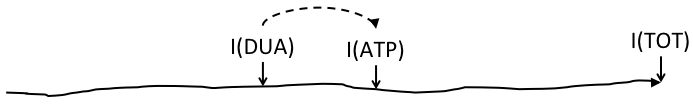
\includegraphics[width=3in]{trace-dua-atp.png}
\caption{A cartoon representing an entire program trace, annotated with instruction count at which DUA is siphoned off to be used, $I(DUA)$, attack point where it is used, $I(ATP)$, and total number of instructions in trace, $I(TOT)$.}
\label{fig:dua-atp-trace}
\end{figure}

The intended use of the bugs created by this system is as ground truth for development and evaluation of vulnerability discovery tools and techniques. 
Thus, it is crucial that they be realistic in some sense.  
Realism is, however, difficult to assess.

Because this work is, to our knowledge, the first to consider the problem of fully automated bug injection, we are not able to make use of any standard measures for bug realism.
Instead, we devised our own measures, focusing on features such as how well distributed the malformed data input and trigger points were in the program's execution, as well as how much of the original behavior of the program was preserved.

We examined three aspects of our injected bugs as measures of realism. 
The first two are DUA and attack point position within the program trace, which are depicted in Figure~\ref{fig:dua-atp-trace}.
That is, we determined the fraction of trace instructions executed at the point the DUA is siphoned off and at the point it is used to attack the program by corrupting an internal program value.

Histograms for these two quantities, $I(DUA)$ and $I(ATP)$, are provided in Figures~\ref{fig:dua-hist} and~\ref{fig:atp-hist}, where counts are for all potential bugs in the LAVA database for all five open source programs. 
DUAs and attack points are clearly available at all points during the trace, although there appear to be more at the beginning and end.
This is important, since bugs created using these DUAs have entirely realistic control and data-flow all the way up to $I(DUA)$.
Therefore, vulnerability discovery tools will have to reason correctly about all of the program up to $I(DUA)$ in order to correctly diagnose the bug.

Our third metric concerns the portion of the trace \emph{between} the $I(DUA)$ and $I(ATP)$.
This segment is of particular interest since LAVA currently makes data flow between DUA and attack point via a pair of function calls.
Thus, it might be argued that this is an unrealistic portion of the trace in terms of data flow.
The quantity $I(DUA)/I(ATP)$ will be close to 1 for injected bugs that minimize this source of unrealism.
This would correspond to the worked example in Figure~\ref{fig:worked-example}; the DUA is still in scope when, a few lines later in the same function, it can be used to corrupt a pointer.
No abnormal data flow is required.
The histogram in Figure~\ref{fig:rdf-hist} quantifies this effect for all potential LAVA bugs, and it is clear that a large fraction have $I(DUA)/I(ATP) \approx 1$, and are therefore highly realistic by this metric.

\begin{figure}
\centering
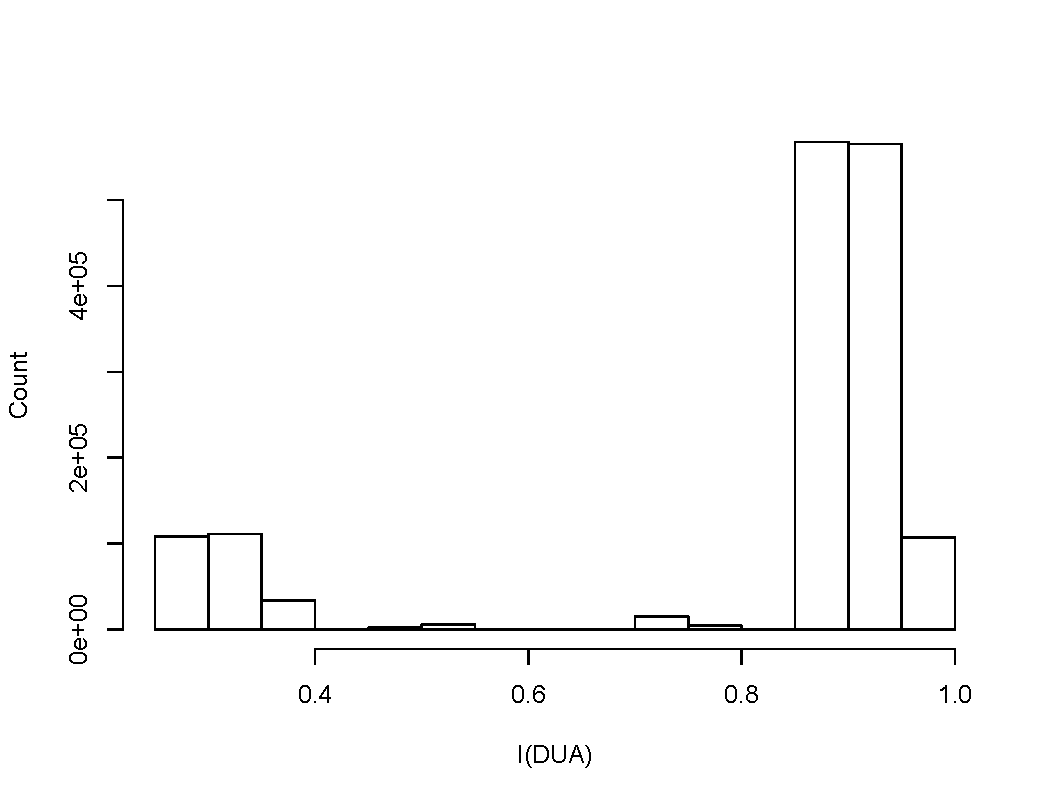
\includegraphics[width=3in]{dua.pdf}
\caption{Normalized DUA trace location}
\label{fig:dua-hist}
\end{figure}

\begin{figure}
\centering
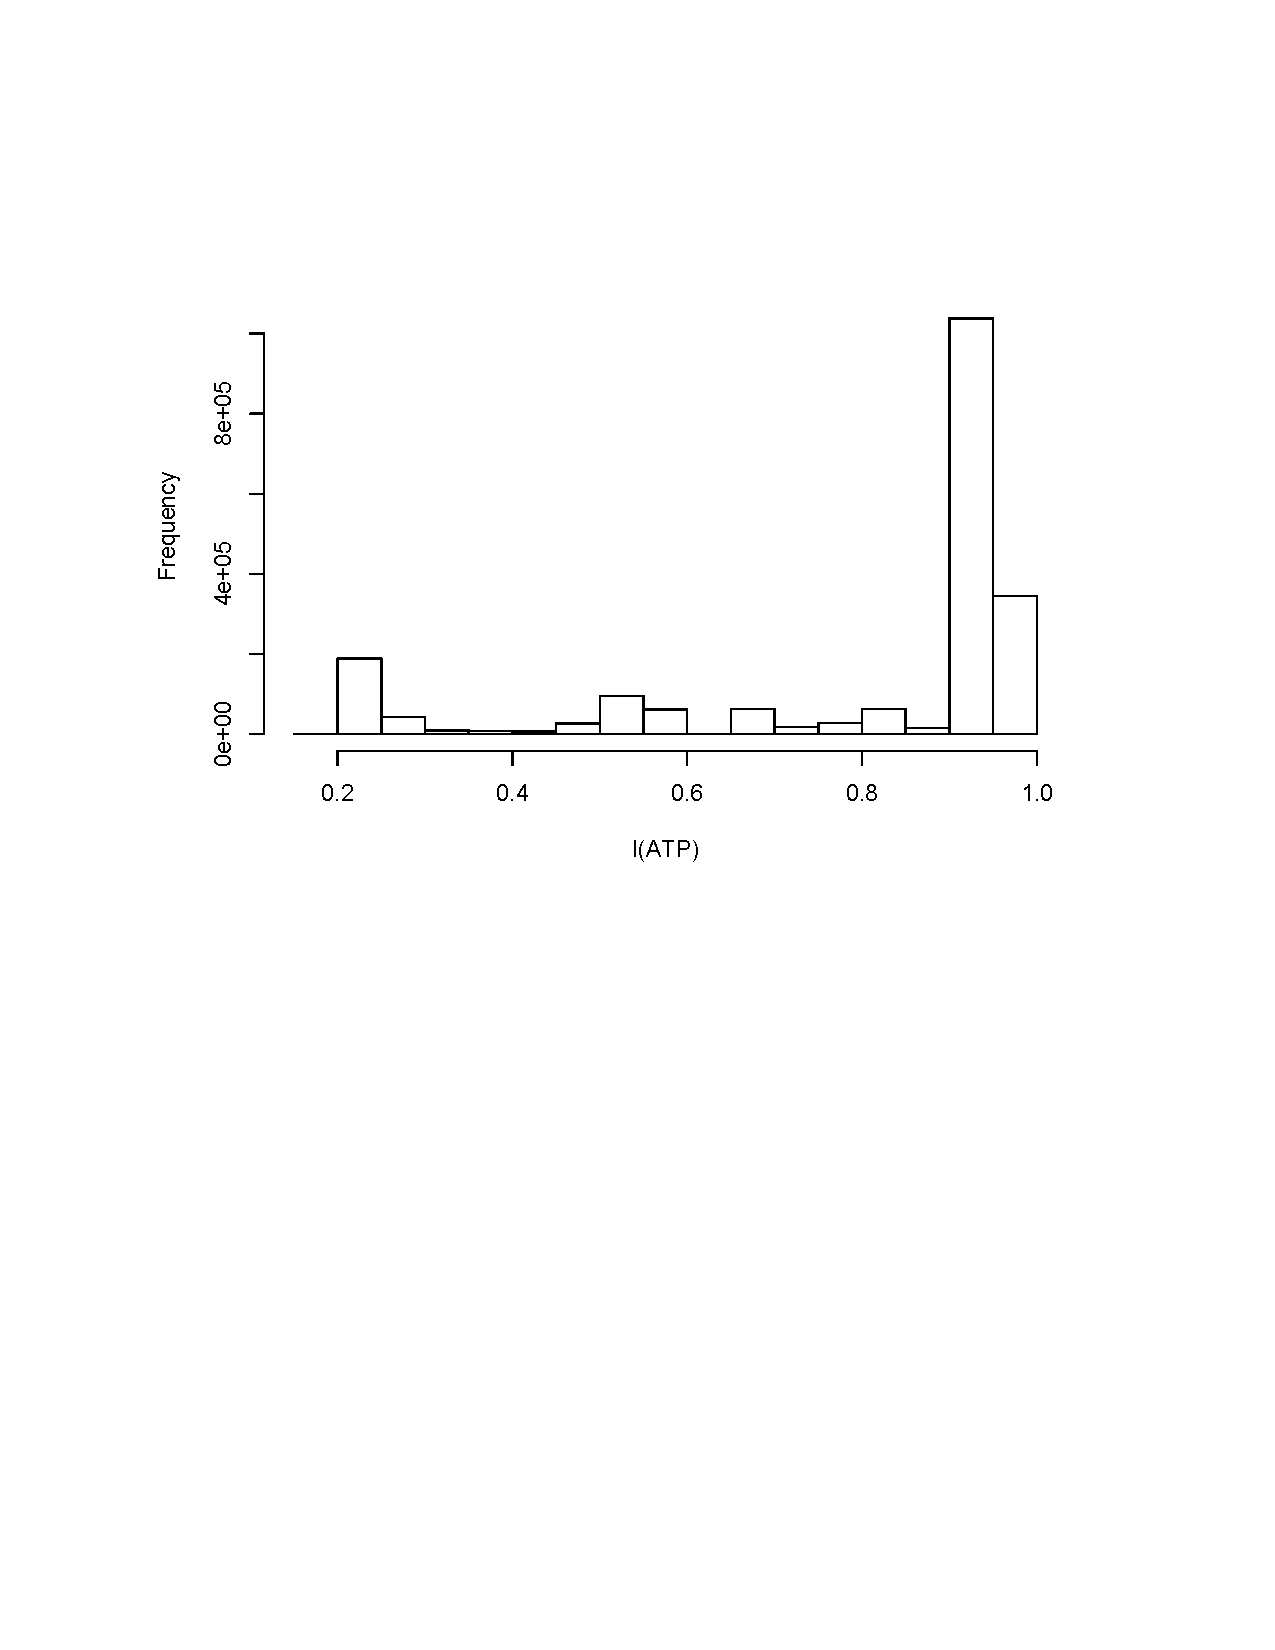
\includegraphics[width=3in]{atp.pdf}
\caption{Normalized ATP trace location}
\label{fig:atp-hist}
\end{figure}

\begin{figure}
\centering
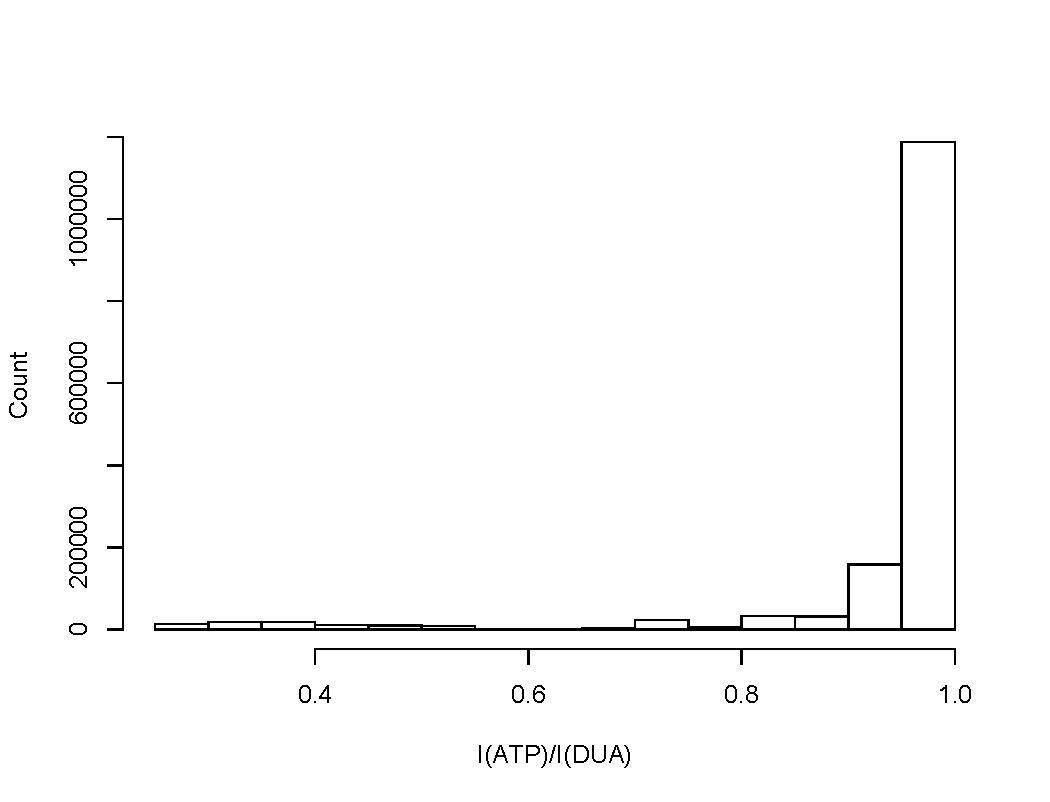
\includegraphics[width=3in]{rdf.pdf}
\caption{Fraction of trace with perfectly normal or realistic data flow, $I(DUA)/I(ATP)$}
\label{fig:rdf-hist}
\end{figure}




\subsection{Vulnerability Discovery Tool Evaluation}

We ran two vulnerability discovery tools on LAVA-injected bugs to investigate their use in evaluation.

\begin{enumerate}
\item Coverage guided fuzzer (referred to as FUZZER)
\item Symbolic execution + SAT solving (referred to as SES)
\end{enumerate}

These two, specifically, were chosen because fuzzing and symbolic execution are extremely popular techniques for finding real-world bugs.
FUZZER and SES are both state-of-the-art, high-profile tools. 
For each tool, we expended significant effort to ensure that we were using them correctly.
This means carefully reading all documentation, blog posts, and email lists.
Additionally, we constructed tiny example buggy programs and used them to verify that we were able to use each tool at least to find known easy bugs.  

Note that the names of tools under evaluation are being withheld in reporting results.
Careful evaluation is a large and important job, and we would not want to give it short shrift, either in terms of careful setup and use of tools, or in presenting and discussing results.
Our intent, here, is to determine if LAVA bugs \emph{can be used} to evaluate bug finding systems. 
It is our expectation that in future work either by ourselves or others, full and careful evaluation of real, named tools will be performed using LAVA.
While that work is outside the scope of this paper, we hope to indicate that it should be both possible and valuable. 
Additionally, it is our plan and hope that LAVA bugs will be made available in quantity and at regular refresh intervals for self-evaluation and hill climbing.

The first corpus we created, \emph{LAVA-1}, used the \verb+file+ target, the smallest of those programs into which we have injected bugs.
This corpus consists of sixty-nine buffer overflow bugs injected into the source with LAVA, each on a different branch in a \verb+git+ repository with a fuzzed version of the input verified to trigger a crash checked in along with the code.
Two types of buffer overflows were injected, each of which makes use of a single 4-byte DUA to trigger and control the overflow.

\begin{enumerate}
    \item \textbf{Knob-and-trigger}. 
In this type of bug, two bytes of the DUA (the \emph{trigger}) are used to test against a magic value to determine if the overflow will happen.
The other two bytes of the DUA (the \emph{knob}) determine how much to overflow. 
Thus, these bugs manifest if a 2-byte unsigned integer in the input is a particular value but only if another 2-bytes in the input are big enough to cause trouble. 
    \item \textbf{Range}. 
These bugs trigger if the magic value is simply in some range, but also use the magic value to determine how much to overflow.
The magic value is a 4-byte unsigned integer and the range varies.  
\end{enumerate}

These bug types were designed to mirror real bug patterns.  
In knob-and-trigger bugs, two different parts of the input are used in different ways to determine the manifestation of the bug.  
In range bugs, rather than triggering on a single value out of $2^{32}$, the size of the haystack varies.
Note that a range of $2^0$ is equivalent to the bug presented in Figure~\ref{src:dua-use}.

\begin{table}[h]
\caption{Percentage of bugs found in \emph{LAVA-1} corpus} %. % as a function of $Bug Type$ and $Tool Type$.  
\centering\footnotesize
\begin{tabular}{l|l|l|l|l|l|l} 
Tool   &                     \multicolumn{6}{|c}{Bug Type}                           \\  \hline  
         &                     \multicolumn{5}{|c|}{Range}                   &     \\   
         &    $2^0$   & $2^7$       & $2^{14}$     & $2^{21}$   & $2^{28}$     & KT   \\  \hline 
FUZZER &    0       & 0           & 9\%          & 79\%       & 75\%         & 20\%      \\
%$CSA_1$ &    0       & 0           & 0            & 0          & 0            & 0         \\
SES    &    8\%     & 0           & 9\%          & 21\%       & 0            & 10\%         \\
\end{tabular}
%\caption{Percentage of bugs found in \emph{LAVA-1} corpus. % as a function of $Bug Type$ and $Tool Type$.  
%FUZZER proved to be an effective vulnerability finding tool.
%However, it was only able to find bugs that allowed an enormous range of possible inputs to trigger the bug.}
\label{table:eval1-file}
\end{table}

The results of this evaluation are summarized in Table~\ref{table:eval1-file}.
Ranges of five different sizes were employed: $2^0, 2^7, 2^{14}, 2^{21}, 2^{28}$. 
We examined all output from both tools.
FUZZER ran for five hours on each bug and found bugs in the larger ranges ($2^{14}$, $2^{21}$, and $2^{28}$).
It was also able to uncover 20\% of the knob-and-trigger bugs, perhaps because the knob and trigger could be fuzzed independently.
SES ran for five hours on each bug, and found several bugs in all categories except the $2^7$ and $2^{28}$ ranges.

The results for the \emph{LAVA-1} corpus seem to accord well with how these tools work.
FUZZER uses the program largely as a black box, randomizing individual bytes, and guiding exploration with coverage measurements.
Bugs that trigger if and only if a four-byte extent in the input is set to a magic value are unlikely to be discovered in this way.
Given time, FUZZER finds bugs that trigger for large byte ranges. 
Note that for many of these LAVA bugs, when the range is so large, discovery is possible by simply fuzzing every byte in the input a few times.  
These bugs may, in fact, be trivially discoverable with a regression suite for a program like \verb+file+ that accepts arbitrary file input.\footnote{In principle, anyway. In practice \texttt{file}'s test suite consists of just 3 tests, none of which trigger our injected bugs.}
By contrast, SES is able to find both knob-and-trigger bugs and different ranges, and the size of the range does not affect the number of bugs found.
This is because it is no more difficult for a SAT solver to find a satisfying input for a large range than a small range; rather, the number of bugs found is limited by how deep into the program the symbolic execution can go.

Note that having each bug in a separate copy of the program means that for each run of a bug finding tool, only one bug is available for discovery at a time.  
This is one kind of evaluation, but it seems to disadvantage tools like FUZZER and SES, which appear to be designed to work for a long time on a single program that may contain multiple bugs. 

Thus, we created a second corpus, \emph{LAVA-M}, in which we injected more than one bug at a time into the source code.
We chose four programs from the \verb+coreutils+ suite that took file input: \verb+base64+, \verb+md5sum+, \verb+uniq+, and \verb+who+.
Into each, we injected as many verified bugs as possible.
Because the \verb+coreutils+ programs are quite small, and because we only used a single input file for each to perform the taint analysis, the total number of bugs injected into each program was generally quite small.
The one exception to this pattern was the \verb+who+ program, which parses a binary file with many dead or even unused fields, and therefore had many DUAs available for bug injection.

We were not able to inject multiple bugs of the two types described above (knob-and-trigger and range) as interactions between bugs became a problem, and so all bugs were of the type in Figure~\ref{src:dua-use}, which trigger for only a single setting of four input bytes.  
The \emph{LAVA-M} corpus, therefore, is four copies of the source code for \verb+coreutils+ version 8.24.
One copy has 44 bugs injected into \verb+base64+, and comes with 44 inputs known to trigger those bugs individually.
Another copy has 57 bugs in \verb+md5sum+, and a third has 28 bugs in \verb+uniq+.
Finally, there is a copy with 2136 bugs existing all at once and individually expressible in \verb+who+.


\begin{table}[h]
\caption{Bugs found in \emph{LAVA-M} corpus by tool type}
\centering\footnotesize
\begin{tabular}{l|c|c|c|c} 
\multirow{2}{*}{Tool Name} & \multirow{2}{*}{Total Bugs} & \multicolumn{3}{c}{Unique Bugs Found} \\
              &            & FUZZER       & SES        & Combined \\ \hline 
\verb+uniq+   &    28      & 7            & 0          & 7               \\
\verb+base64+ &    44      & 7            & 9          & 14               \\
\verb+md5sum+ &    57      & 2            & 0          & 2               \\
\verb+who+    &    2136    & 0            & 18         & 18               \\
Total         &    2265    & 16           & 27         & 41               \\
\end{tabular}
\label{table:tool-eval-results-coreutils}
\end{table}

We ran FUZZER and SES against each program in \emph{LAVA-M}, with 5 hours of runtime for each program.
\verb+md5sum+ ran with the \verb+-c+ argument, to check digests in a file.
\verb+base64+ ran with the \verb+-d+ argument, to decode base 64.

SES found no bugs in \verb+uniq+ or \verb+md5sum+.
In \verb+uniq+, we believe this is because the control flow is too unconstrained.
In \verb+md5sum+, SES failed to execute any code past the first instance of the hash function.
\verb+base64+ and \verb+who+ both turn out more successful for SES.
The tool finds 9 bugs in \verb+base64+ out of 44 inserted; these include both deep and shallow bugs, as \verb+base64+ is such a simple program to analyze.

SES's results are a little more complicated for \verb+who+.
All of the bugs it finds for \verb+who+ use one of two DUAs, and all of them occur very early in the trace.
One artifact of our method for injecting multiple bugs simultaneously is that multiple bugs share the same attack point.
It is debatable how well this represents real bugs.
In practice, it means that SES can only find one bug per attack point, as finding an additional bug at the same attack point does not necessarily require covering new code.
LAVA could certainly be changed to have each bug involve new code coverage.
SES could also be improved to find all the bugs at each attack point, which means generating multiple satisfying inputs for the same set of conditions.

FUZZER found bugs in all utilities except \verb+who+.\footnote{In fact, we allowed FUZZER to continue running after 5 hours had passed; it managed to find a bug in \texttt{who} in the sixth hour.}
Unlike SES, the bugs were fairly uniformly distributed throughout the program, as they depend only on guessing the correct 4-byte trigger at the right position in the input file.

FUZZER's failure to find bugs in \verb+who+ is surprising.
We speculate that the size of the seed file (the first 768 bytes of a \verb+utmp+ file) used for the fuzzer may have been too large to effectively explore through random mutation, but more investigation is necessary to pin down the true cause.
Indeed, tool anomalies of this sort are exactly the sort of thing one would hope to find with LAVA, as they represent areas where tools might make easy gains.

We note that the bugs found by FUZZER and SES have very little overlap (only 2 bugs were found by both tools).
This is a very promising result for LAVA, as it indicates that the kinds of bugs created by LAVA are not tailored to a particular bug finding strategy.

%We also evalued a second commercial static analyzer, referred to in this text as $CSA_2$. Because we were only allowed a limited number of analysis runs, we opted to create a single version of \verb+who+ from the GNU coreutils that contained 60 injected, verified bugs. This was fed to $CSA_2$, generating 117 alerts; we then went through its alerts by hand to see which ones referenced our injected bugs.

%Of the 117 alerts, 17 referred to code we had injected into \verb+who+. We did not investigate the other 100 further; presumably these are some mix of true and false positives in the original source code to \verb+who+. The 17 that were specific to our injected bugs were examined in more detail. Fourteen were found to be essentially false positives: they referred to innocuous artifacts of the injection process. For example, to guard against introducing pointer errors, we emit code like \verb+if(p) { ... }+; however, the static analysis software took this as proof that \verb+p+ might be NULL, and then warned us that it was dereferenced elsewhere before the NULL check. After discounting such artifacts, we found that $CSA_2$ correctly identified three of our injected bugs, labeling them all as ``Out-of-bounds access''.


\section{Related Work}
\label{sec:relwork}
The design of LAVA is driven by the need for bug corpora that are a)
dynamic (can produce new bugs on demand), b) realistic (the bugs occur
in real programs and are triggered by the program's normal input), and
c) large (consist of hundreds of thousands of bugs). In this section we
survey existing bug corpora and compare them to the bugs produced by
LAVA.

The need for realistic corpora is well-recognized. Researchers have
proposed creating bug corpora from student code~\cite{Spacco:2005},
drawing from existing bug report databases~\cite{Lu:2005,Meftah:2005},
and creating a public bug registry~\cite{Foster:2005}. Despite these
proposals, public bug corpora have remained static and relatively small.

The earliest work on tool evaluation via bug corpora appears to be by
Wilander and Kamkar, who created a synthetic testbed of 44 C function
calls~\cite{Wilander:2002} and 20 different buffer overflow
attacks~\cite{Wilander:2003} to test the efficacy of static and dynamic
bug detection tools, respectively. These are synthetic test cases,
however, and may not reflect real-world bugs. In 2004, Zitser et
al.~\cite{Zitser:2004} evaluated static buffer overflow detectors; their
ground truth corpus was painstakingly assembled by hand over the course
of six months and consisted of 14 annotated buffer overflows with
triggering and non-triggering inputs; these same 14 overflows were later
used to evaluate dynamic overflow detectors~\cite{Zhivich:2005}.
Although these are real bugs from actual software, 

The most extensive effort to assemble a public bug corpus comes from the
NIST Software Assurance Metrics And Tool Evaluation (SAMATE)
project~\cite{Kass:2005}. Their evaluation corpus inclues
Juliet~\cite{Juliet:2012}, a collection of 86,864 synthetic C and Java
programs that exhibit 118 different CWEs; each program, however, is
relatively short and has uncomplicated control \& data flow. The corpus
also includes the IARPA STONESOUP data set~\cite{SAMATE:2014}, which was
developed in support of the STONESOUP vulnerability mitigation project.
The test cases in this corpus consist of 164 small snippets of C and
Java code, which are then spliced into program to inject a bug. The bugs
injected in this way, however, do not use the original input to the
program (they come instead from extra files and environment variables
added to the program), and the data flow between the input and the bug
is quite short.

Finally, the general approach of automatic program transformation to
introduce errors was also used by Rinard et al.~\cite{Rinard:2005}; the
authors systematically modified the termination conditions of loops to
introduce off-by-one errors in the Pine email client to test whether
software is still usable in the presence of errors once sanity checks
and assertions are removed.



\section{Limitations and Future Work}
\label{sec:future}
%Limitations:
%- C code only
%- Dataflow is... manufactured, maybe not reflective
%- Limited class of bugs (pointer corruptions)
% bug injection artifacts due to no actual static analysis

A significant chunk of future work for LAVA involves making the generated corpora look more like more of the bugs that are found in real programs. 
LAVA currently injects only buffer overflows into programs.
But our taint-based analysis overcomes the crucial first hurdle to injecting any kind of bug: making sure that attacker-controlled data can be used in the bug's potential exploitation. 
As a result, other classes of bugs, such as temporal safety bugs (use-after-free) and meta-character bugs (e.g. format string) should also be injectable using our approach. 
There also remains work to be done in making LAVA's bug-triggering data flow more realistic, although even in its current state, the vast majority of the execution of the modified program is realistic. 
This execution includes the data flow that leads up to the capture of the DUA, which is often nontrivial.

However rosy the future seems for LAVA, it is likely that certain classes of bugs are simply not injectable via taint-based measures.
Logic errors, crypto flaws, and side-channel attacks, for instance, all seem to operate at a rather different level than the kinds of data-flow triggered flaws LAVA is well positioned to generate.
We are not hopeful that these types of vulnerabilities will soon be injectable with LAVA. 

We discovered, in the course of our use of LAVA bugs to evaluate vulnerability discovery tools, a number of situations in which LAVA introduces unintended bugs, such as use-after free and dereference of an uninitialized pointer in the code that siphons of a DUA value for later use triggering a bug.  
In some cases, the tool under evaluation even found these real bugs that were due to LAVA artifacts and we had to remove them and re-run in order to ensure that the evaluation was not compromised. 
These artifacts are a result of LAVA performing no real static analysis to determine if it is even vaguely safe to dereference a pointer in order to introduce the data flow it requires to inject a bug.
It should be possible to remedy this situation dramatically in many cases but a complete solution would likely require intractable whole-program static analysis.  

LAVA is limited to only work on C source code, but there is no fundamental reason for this.
In principle, our approach would work for any source language with a usable source-to-source rewriting framework. 
In Python, for example, one could easily implement our taint queries in a CPython plugin that executed the hypervisor call against the address of a variable in memory. 
Since our approach records the correspondence between source lines and program basic block execution, it would be just as easy to figure out where to edit the Python code as it is in C.
We have no immediate plans to extend LAVA in these directions.

We are planning some additional evaluatory work.  
In particular, an extensive evaluation of real, named tools should be undertaken and the results examined with care and used to diagnose the the strengths and weaknesses of both implementations and also classes of techniques.
It should also be noted that, in our preliminary evaluation of vulnerability discovery tools, we measured only the \emph{miss rate}; no attempt was made to gauge the \emph{false alarm rate}.
It is not clear exactly how LAVA can be used to measure false alarms for every kind of tool.
For tools that generate a triggering input, as do both SES and FUZZER, this should be trivial. 
Every input can be tested against the program after it has been instrumented to be able to detect the vulnerability.
In the case of buffer overflows in C, this could mean compiling in fine-grained bounds checking~\cite{ruwase2004practical}.
However, many bug finding tools, especially static analyzers and abstract interpretation ones, do not generate existence proof inputs.
Instead, they merely gesture at a line in the program and make a claim about possible bugs at that point.
In this situation, we can think of no way to assess false alarm rate.



\section{Conclusion}
In this paper, we have introduced LAVA, a fully automated system that can rapidly inject large numbers of realistic bugs into C programs.
LAVA has already been used to introduce over 4000 realistic buffer overflows into open-source Linux C programs of up to 2 million lines of code.  
We have used LAVA corpora to evaluate the detection powers of state-of-the-art bug finding tools.
The taint-based measures employed by LAVA to identify attacker-controlled data for use in creating new vulnerabilities are powerful and should be usable to inject many and diverse vulnerabilities, but there are likely fundamental limits; LAVA will not be injecting logic errors into programs anytime soon.
Nevertheless, LAVA is ready for immediate use as an on-demand source of realistic ground truth vulnerabilities for classes of serious vulnerabilities that are still abundant in mission-critical code.
It is our hope that LAVA can drive both development and evaluation of tools and techniques for vulnerability discovery.

%LAVA is fast, injecting a new buffer overflow into a program like \verb+file+ in less than 20 seconds.



\bibliographystyle{plain}
\bibliography{biblio}

\end{document}
